\section{Multivariate Calculus}
Often when considering different machine learning techniques we will consider high dimensional functions $f:\R^d\rightarrow\R$. Usually, these functions will represent some distance measurement between our estimated prediction and the true values. As such, we would like to solve the optimization problem of minimizing this distance. Namely:
$$\underset{{\w\in \R^d}}{argmin}\, f\left(\w\right)$$

\subsection{Derivatives, Gradients and Jacobians}
\subsubsection{Derivatives}
A common approach for finding such a minimizer is by computing the derivative of the function, equating to zero and solving for our parameters $\w$. When discussing multivariate functions we use gradients rather than scalar derivatives.

\begin{definition}[Derivative]
Let $f:\R\rightarrow\R$. The derivative of $f$ at point $x\in\R$ is defined as $$ \frac{d}{dx}f\left(x\right) \coloneqq\lim_{a\rightarrow0}\frac{f\left(x+a\right)-f\left(x\right)}{a} $$
\end{definition}

\begin{example}[ReLU]
Consider the \textbf{Re}ctified \textbf{L}inear \textbf{U}nit function defined as the positive part of its argument: $f\left(x\right) = x^{+} = \max\left(0, x\right)$. This function is in common use in the context of artificial neural networks. The derivative if this function is:
	$$\frac{df\left(x\right)}{dx}=\begin{cases}
		0 & x<0\\
		1 & x>0
	\end{cases}$$	
\end{example}

Note that at $x=0$ the derivative of ReLU is undefined. We will discuss ways to handle such cases in \autoref{chap:conv_opt}. Next, let us expand the derivative definition to multivariate functions.

\begin{definition}[Partial Derivative]
Let $f:\R^d\rightarrow\R$. The partial derivative of $f$ at point $\x\in\R^d$ with respect to $x_{i}$ is defined as
\begin{align*}
	\frac{\partial}{\partial x_{i}} f\left(\x\right) & \coloneqq \lim_{a\rightarrow0}\frac{f\left(\x+a\mathbf{e}_{i}\right)-f\left(\x\right)}{a}\\
	& =\lim_{a\rightarrow0}\frac{f\left(x_{1},\dots,x_{i}+a,\dots,x_{d}\right)-f\left(x_{1},\dots,x_{i},\dots,x_{d}\right)}{a}
\end{align*}
where $\mathbf{e}_{i}$ is the $i$-th standard basis vector. 
\end{definition}

Namely, a partial derivative of a function is its derivative with respect to one of its variables, while all others are kept constant. 

\begin{example}[Max]
For $f\left(\x\right) = max_i\left(x_1,\ldots,x_d\right)$ the partial derivatives of $f$ at $x_i$ are:
$$ \frac{\partial}{\partial x_i}f\left(\x\right) = \begin{cases}
	1 & i=argmax\left(x_{1},\ldots,x_{d}\right)\\
	0 & i\neq argmax\left(x_{1},\ldots,x_{d}\right)
\end{cases} $$
\end{example}

\begin{figure}[H]
	\centering
	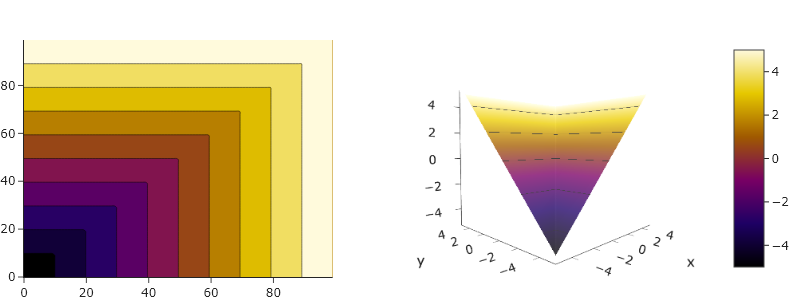
\includegraphics[width=0.8\textwidth]{chapters/mathematical.basis/figures/max.png}
	\caption{Visualization of bi-variate $max$ function in 3D and 2D. \GitChapterOneExamples}
\end{figure}


\begin{example}[Polynomial]
For $f\left(x,y\right) = x^2 + xy + y^2$ the partial derivatives of $f$ at $\left(x_0,y_0\right)$ are  $$\frac{\partial}{\partial x}f\left(x_0,y_0\right)=2x_0+y_0, \quad\frac{\partial}{\partial y}f\left(x_0,y_0\right)=2y_0+x_0$$
\end{example}

\begin{figure}[H]
	\centering
	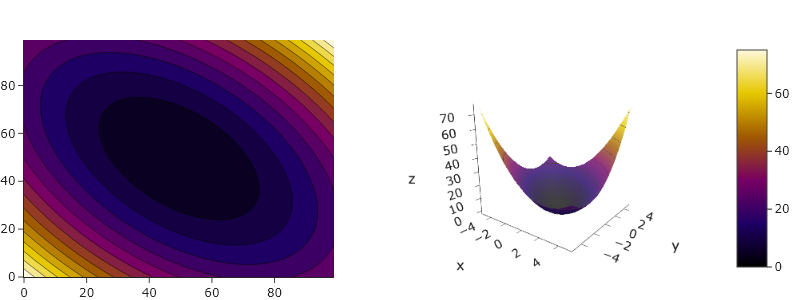
\includegraphics[width=0.8\textwidth]{chapters/mathematical.basis/figures/polynomial.png}  
	\caption{Visualization of bi-variate polynomial of degree 2 in 3D and 2D. \GitChapterOneExamples}
\end{figure}
 
\subsubsection{Gradients}
\begin{definition}[Gradient]
The gradient of $f$ at $\x$ is the vector of partial derivatives:
$$\nabla f\left(\x\right) \coloneqq \left(\frac{\partial f\left(\x\right)}{\partial x_1},\ldots, \frac{\partial f\left(\x\right)}{\partial x_d} \right)^\top $$
\end{definition}


\begin{example}\label{exe:gradient_poly}
By using the partial derivatives previously calculated of a second order bivariate polynomial $f\left((x,y\right)=x^2 + xy + y^2$, the gradient of $f$ at $\x_0=\left(x_0,y_0\right)$ is  $$\nabla f\left(\x_0\right) = \left(2x_0+y_0, 2y_0+x_0\right)^\top.$$
\end{example}

\begin{exercise}[Linear Functional]\label{exe:linear_functional}
Let $\w\in\R^d$ and $f:\R^d\rightarrow\R$ defined as $f\left(\x\right)=\w^\top\x$. Compute the gradient of $f$ at point $\x$.
\end{exercise}
\begin{proof}
From linearity of the derivative:
$$ \frac{\partial}{\partial x_j}f\left(\x\right) = \sum_i \frac{\partial}{\partial x_j}f\left(\x\right)_i = \sum \frac{\partial}{\partial x_j} \w_i\x_i = \w_j  $$
Therefore, in vector notation $\nabla f\left(\x\right) = \w$.
\end{proof}

\begin{exercise}[Norm]\label{exe:grad_norm}
Let $f:\R^d\rightarrow\R$ be defined by $f\left(\x\right) = \norm{\x}^2$. Compute the gradient of $f$ at point $\x$.
\end{exercise}
\begin{proof}
Similar to the previous exercise, using the linearity of the derivative then:

$$ \frac{\partial}{\partial x_j} f\left(x\right) = \sum_i \frac{\partial}{\partial x_j} x_i^2 = 2x_j $$
which in vector notation can be written as: $\nabla f\left(\x\right) = 2\x$.
\end{proof}


\subsubsection{Jacobians}
In different applications in machine learning, the function we are trying to minimize is a vector-valued function, namely $f:\R^m\rightarrow\R^d$. 

~\\ For example, consider the following scenario. We have gathered historic information of season, time of day, latitude and longitude at different points in the world. Next, we have described some function that given these parameters states the temperature and air-pressure of that location and time. We want to find the the extrema points of this function. In this scenario, the described function gets fours parameters and returns two outputs $f:\R^4\rightarrow\R^2$. In order to find the extrema points we need to generalize the gradient definition to vector-valued functions.
~\\
\begin{definition}[Jacobian]
	Let $\vv{f}:\R^m\rightarrow\R^d$ where $\vv{f}\left(\x\right)=\left(f_1\left(\x\right),\ldots, f_d\left(\x\right)\right)^\top$. The Jacobian of $f$ is the $d\times m$ matrix of all partial derivatives:
	\[
	J_{\x}\left(\vv{f}\right)\coloneqq\begin{bmatrix}\frac{\partial f_{1}\left(\x\right)}{\partial x_1} & \ldots & \frac{\partial f_1\left(\x\right)}{\partial x_m}\\
		\vdots &  & \vdots\\
		\frac{\partial f_d\left(\x\right)}{\partial x_1} & \ldots & \frac{\partial f_d\left(\x\right)}{\partial x_m}
	\end{bmatrix}
	\]
\end{definition}

\begin{example}
Let us revisit \autoref{exe:gradient_poly} where $f:\R^2\rightarrow\R$ defined as $f\left(\x\right)=x_1^2+x_2^2$. The Jacobian of $f$ is:
$$ J_{\\x}\left(\vv{f}\right)=\left[\begin{array}{cc}
	\frac{\partial f_1\left(\x\right)}{\partial x_1} & \frac{\partial f_1\left(\x\right)}{\partial x_2}\end{array}\right]=\left[2x_1,2x_2\right]=\nabla f\left(\x\right)^\top $$
\end{example}

Notice that for any function where $k=1$ the Jacobian is infact the transposed gradient vector: $J_{\x}\left(f\right)=\nabla f\left(\x\right)^\top$.

\begin{exercise}\label{exe:lin_jcob}
Let $A\in\R^{m\times d}$ and let $f:\R^d\rightarrow\R^m$ defined as $f\left(\x\right)=A\x$.  Find the Jacobian of $f$: $J_{\x}\left(f)\right)$.
\end{exercise}
\begin{proof}
Let us define the set of functions computing each coordinate in the output vector $\forall i\in\left[d\right]\quad f_i\left(\x\right)=A_i^\top \x$. Then the jacobian of $f$ is comprised of the gradients of $f_1,\ldots, f_d$ as rows. Notice that we have already computed the gradient of linear functionals in \autoref{exe:linear_functional} so:
$$ J_{\x}\left(f\right)=\left[\begin{array}{c}
	\nabla f_{1}\left(\x\right)^{\top}\\
	\vdots\\
	\nabla f_{d}\left(\x\right)^{\top}
\end{array}\right]=\left[\begin{array}{c}
	-A_{1}-\\
	\vdots\\
	-A_{d}-
\end{array}\right]=A $$
\end{proof}

\subsubsection{Chain Rules}
\begin{theorem}[Chain Rule - Univariate]
Let $f:\R\to\R$ and $g:\R\to\R$ be two differential functions, then the derivative of the composite $f\circ g$ is: $$ \left(f\circ g\right)' \coloneqq \left(f'\circ g\right)\cdot g' $$
Namely, for $h\left(x\right)=f\left(g\left(x\right)\right)$ then $\forall x\in\R$ $h'\left(x\right)=f'\left(g\left(x\right)\right)\cdot g'\left(x\right)$.
\end{theorem}

\begin{theorem}[Chain Rule - Multivariate]
Let $f:\R^d\rightarrow\R^m$ and $g:\R^k\rightarrow\R^d$. The Jacobian of the composition $\left(f\circ g\right):\R^k\rightarrow\R^m$ at $\x$ is 
$$
J_{\x}\left(f\circ g\right) = J_{g\left(\x\right)}(f)J_{\x}\left(g\right) 
\coloneqq\begin{bmatrix}
	\frac{\partial f_1\left(g\left(\x\right)\right)}{\partial g_1\left(\x\right)} & \ldots & \frac{\partial f_1\left(g\left(\x\right)\right)}{\partial g_d\left(\x\right)}\\
	\vdots &  & \vdots\\
	\frac{\partial f_m\left(g\left(\x\right)\right)}{\partial g_1\left(\x\right)} & \ldots & \frac{\partial f_m\left(g\left(\x\right)\right)}{\partial g_d\left(\x\right)}
\end{bmatrix}
=\begin{bmatrix}\frac{\partial g_1\left(\x\right)}{\partial x_1} & \ldots & \frac{\partial g_1\left(\x\right)}{\partial x_k}\\
	\vdots &  & \vdots\\
	\frac{\partial g_d\left(\x\right)}{\partial x_1} & \ldots & \frac{\partial g_d\left(\x\right)}{\partial x_k}
\end{bmatrix}
$$
In element-wise notation:  $$J_{\x}\left(f\circ g\right)_{i,j} \coloneqq \sum_l\frac{\partial f_i\left(g\left(\x\right)\right)}{\partial g_l\left(\x\right)}  \frac{\partial g_l\left(\x\right)}{\partial x_j} $$
\end{theorem}

\begin{exercise}
Let $f\left(\x\right)=\norm{\x}^2$ and $g\left(\x\right)=A\x$ for some matrix $A\in\R^{m\times d}$. Calculate the jacobian of $f\circ g$.
\end{exercise}
\begin{proof}
From the previous theorem we know that:
$$ J_{\x}\left(f\circ g\right) = J_{g\left(\x\right)}\left(f\right)J_\x\left(g\right)$$
As $g$ a linear transformation we have see in \autoref{exe:lin_jcob} that $J_\x\left(g\right)=A$. Notice, that as $Im\left(f\right)\subseteq \R$, the jacobian of $f$ equals to the transpose of its grad	ient. As seen in \autoref{exe:grad_norm}, $J_{g\left(\x\right)}\left(f\right)=\left(2g\left(\x\right)\right)^\top$. Therefore:
$$ J_\x\left(f\circ g\right) = 2\x^\top A^\top A$$
\end{proof}

Next, let us calculate the gradient of the following function: $f\left(\x\right) = \frac{1}{2} \norm{A\x-\y}^2$. Applying the chain rule then:
$$ 
\begin{array}{ccl}
	\nabla f\left(\x\right) & = & \frac{\partial}{\partial \x}\frac{1}{2}\norm{A\x-\y}^2  \\
	& = & \frac{1}{2}\frac{\partial}{\partial \x}\left(\x^\top A^\top A \x - 2\y^\top A\x + \y^\top y\right) \\
	& = & A^\top A \x - A^\top y \\ 
	& = & A^\top\left(A\x-\y\right)
\end{array}$$
This function is known as the Mean Square Error (MSE) and in \autoref{rss} we will use the above derivation in order to find the values of $\x$ that minimize $f$ as above.

\begin{example}[Soft-Max]
The softmax function defined over $S:\R^d \rightarrow \left[0,1\right]^d$ returns a vector that its coordinates sum up to 1. It is defined by $$S\left(\vv{a}\right)_{j}=\frac{e^{a_{j}}}{\sum_{k=1}^{N}e^{a_{k}}}$$

As the coefficients $a_j$ are in the power of the exponent function, all outputted values are strictly positive. Moreover, since the numerator appears in the denominator summed up with some other positive numbers, $S_{j}<1$. Therefore, it is in the range $\left(0,1\right)$. For example, the 3-element vector $(1, 2, 5)$ gets transformed into $(0.02, 0.05, 0.93)$. The order of elements by relative size is preserved, and they add up to 1.0. In addition, the third element is now farther away from the first two, Its softmax value is dominating the overall slice of size 1.0 in the output. ~\\

Intuitively, the $softmax$ function is a "soft" version of the $argmax$ function. Instead of just selecting one maximal element, softmax breaks the vector up into segments with the maximal input element getting a proportionally larger chunk, but the other elements getting some of it as well. Softmax is often used in neural networks, to map the non-normalized output to a probability distribution over predicted output classes.

~\\ Let us calculate the derivative of the softmax function. Denote $g_{i\left(\vv{a}\right)}\coloneqq e^{a_{i}}$  and $h\left(\vv{a}\right)\coloneqq \sum_{k=1}^{N}g_i\left(\vv{a}\right)$. So:
$$\frac{\partial S_{i}}{\partial a_{j}}=\frac{\partial}{\partial a_{j}}\frac{e^{a_{i}}}{\sum_{k=1}^{N}e^{a_{k}}}=\frac{\partial}{\partial a_{j}}\frac{g_{i}}{h}$$

Note that for any $a_j$ the derivative of $h$ is $e^{a_j}$. In the case of $g_i$, when deriving with respect to $a_j$ we get that the derivative is $e^{a_j}$ only if $i=j$. Otherwise, the derivative is $0$. Therefore, the derivative of $S_i$ in the case where $i=j$ is:

$$\frac{\partial}{\partial a_{j}}\frac{e^{a_{i}}}{\sum_{k=1}^{N}e^{a_{k}}} = \frac{e^{a_{i}}({\sum_{k=1}^{N}e^{a_{k}}}) - e^{a_{i}} e^{a_{j}}} {({\sum_{k=1}^{N}e^{a_{k}}})^{2}}=\frac{e^{a_{i}}}{({\sum_{k=1}^{N}e^{a_{k}}})}\cdot\frac{({\sum_{k=1}^{N}e^{a_{k}}})-e^{a_{j}}}{({\sum_{k=1}^{N}e^{a_{k}}})}=S_{i}\left(1-S_{j}\right)$$

It is left to show the derivative in the case where $i\neq j$.
\end{example}

\subsection{First Order Function Approximation}
As motivated in the begining of this section, we are often interested in finding the minimizers of some multivariate objective function. Many times, these functions are very hard, or even impossible, to solve analytically. In such cases we might consider approximating the true function with a simpler one that we are able to solve. 

~\\Consider a function $f:\R\rightarrow\R$ and recall the definition of the Taylor series:
$$T\left(x_0+x\right)=\sum_{n=0}^\infty \frac{f^{\left(n\right)}\left(x_0\right)}{n!}x^n = f\left(x_0\right)+f'\left(x_0\right)x+\frac{1}{2}f''\left(x_0\right)x^2 + \ldots$$
A linear approximation (or first order approximation) is an approximation of a general function using a linear function. For a twice continuously differentiable function $f:\R\rightarrow\R$, Taylor's theorem implies that for small $x$
$$f\left(x_0+x\right) \approx f\left(x_0\right) + f'\left(x_0\right)x$$
We can now extend this theorem to define linear approximations of multivariate functions.

\begin{definition}[Linear Approximation]
Let $f:\R^d\rightarrow\R$ and $\vv{p}_0\in\R^d$. The linear approximation of $f$ for every $\vv{p}$ near $\vv{p}_0$ is defined as $$f\left(\vv{p}_0\right)+\inprod{\nabla f\left(\vv{p}_0\right)}{\vv{p}-\vv{p}_0}$$
	
Equivalently, if we treat $\vv{p}$ as the deviation from $\vv{p}_0$ then: 
$$f\left(\vv{p}_0 + \vv{p}\right)\approx f\left(\vv{p}_0\right)+ \inprod{\nabla f\left(\vv{p}_0\right)}{\vv{p}}$$
\end{definition}

So if for example, we consider a bivariate function $f:\R^2\rightarrow\R$, the linear approximation of $f$ near the point $\left(x_0,y_0\right)$ is:
$$f\left(x_0+x,y_0+y\right)\approx f\left(x_0,y_0\right)+x\cdot\frac{\partial f\left(x_0,y_0\right)}{\partial x}+y\cdot\frac{\partial f\left(x_0,y_0\right)}{\partial y}$$

Now, if $f$ is a linear function, intuition dictates that the linear approximation of $f$ would be the function itself. Let $\vv{b}\in\R^d$ and let $f:\R^d\rightarrow\R$ be defined by $f\left(\x\right)=\vv{b}^\top\x$. Then, the linear approximation of $f$ at $\vv{p}_0$ is
$$ 
\begin{array}{ccl}
f\left(\vv{p}_0\right)+ \inprod{\nabla f\left(\vv{p}_0\right)}{\vv{p}-\vv{p}_0} & =  & \vv{b}^\top \vv{p}_0 + \inprod{\vv{b}}{\vv{p}-\vv{p}_0} \\
& = & \vv{b}^\top\left(\vv{p}_0+\vv{p}-\vv{p}_0\right) = f\left(\vv{p}\right)
\end{array}
$$

\begin{exercise}
Let $f:R^2\rightarrow\R$ be defined by $f\left(x,y\right)= \sqrt{x^2+y^2}$. Calculate the linear approximation of $f$ near $\left(3,4\right)$.
\end{exercise}
\begin{proof}
We begin with expressing the gradient of $f$. So, the partial derivative of $f$ with respect to first argument at point $x$ is:
$$ \frac{\partial}{\partial x} = f\left(x_0,y_0\right) = 2x_0 \cdots \frac{1}{2\sqrt{x_0^2+y_0^2}} $$
Therefore the gradient of $f$ is $\nabla f\left(\x\right) = \left(\frac{x_0}{\sqrt{x_0^2+y_0^2}},\frac{y_0}{\sqrt{x_0^2+y_0^2}}\right)^\top$.
So for a point $\left(x,y\right)$ in the vicinity of $\left(3,4\right)$ the linear approximation is:

$$ f\left(3+x, 4+y\right) \approx 5+\frac{3}{5}x+\frac{4}{5}y$$ 

If for example $x=0.1, y=0.2$ then $f\left(3+0.1,4+0.2\right) = 5.2201.. \approx 5.22 = 5+3/5 \cdot 0.1+4/5 \cdot 0.2$
\end{proof}


Another use of first order approximations is as follows. Suppose we investigate some objective function $f:\R^d\rightarrow\R$ at point $\vv{p}_0\in\R^d$. Now, we would like to "take a step" in $\R^d$ in the direction where $f$ grows with the fastest rate. That is, we are searching for the direction in space, that if we move in, $f$ grows the most. How can we find such direction?

~\\Recall that $f\left(\vv{p}_0+\vv{p}\right)\approx f\left(\vv{p}_0\right)+\nabla f\left(\vv{p}_0\right)\cdot \vv{p}$. In addition, the angle between $\nabla f\left(\vv{p}_0\right)$ and $\vv{p}$ is $\nabla f\left(\vv{p}_0\right)\cdot \vv{p}=\norm{\nabla f\left(\vv{p}_0\right)}\cdot\norm{\vv{p}} \cos\theta$. As we are only interested in the direction in which to step, and not the step size, let us assume that $\norm{\left(\vv{p}\right)}=1$. Since $\cos x \in \left[-1, 1\right]$, the direction that maximizes $f$ is $\vv{p}_{max}\coloneqq \nabla f\left(\vv{p}_0\right)/\norm{\nabla \left(\vv{p}_0\right)}$. Similarly the direction that minimizes $f$ is $\vv{p}_{min}\coloneqq -\nabla f\left(\vv{p}_0\right)/\norm{\nabla \left(\vv{p}_0\right)}$. So, if we adapt a step-wise approach, for sufficiently small enough steps sizes, for maximizing/minimizing $f$, moving in the direction of the gradient or opposite to the gradient is a good approach. We will revisit this concept in \autoref{chap:conv_opt}